\subsection{System Description}
At a core level, the program consists of three or four main modules, the simulation, the renderer, a shared area and the interface, the system is designed using an object orientated structure for the simulation, renderer and shared and makes use of inheritance to reduce code repetition and simplify the underlying structure.

\paragraph{}
The main objects, render and simulation, are run on different threads, this allows the interface to remain responsive even when their is a heavy load on the simulation thread.

\paragraph{}
The shared area inherits the methods in the base class as virtual functions, these consist of set and get functions which will set and return either the control structure or a pointer container, when a pointer container is set, old data is deleted and it creates a copy of the new data to a new pointer. While it is identical, it is a whole new set of data in order to preserve thread-safety. The shared area makes use of polymorphism to modify the functions in the shared area to include mutual exclusion object

\paragraph{}
In order to simplify the management of the bodies objects and remove the automatic out of scope destruction, the objects are allocated using dynamic allocation, the disadvantage of this is that the memory must be kept under check and properly deallocated when it is no longer required. The system that is in place has been verified to delete bodies correctly and does not present any memory leaks.

\paragraph{}
The simulation thread is synchronised to the generally much slower render thread by the use of a condition variable, this interfaces to a mutex object inside the simulation main function and will pause the thread until it is unlocked by a call to the condition variable in the shared area. This effectively locks the iterations to the frame rate one to one unless the iterations per frame is more than 1. While this will result in variance should the frame rate drop below 60 frames per second, this is very unlikely because of how simplistic the graphics are, the simulation will be far slower than the rendering at any body count required to slow down the rendering even on low end and integrated GPUs.

\paragraph{}
The simulation itself makes use of a simplistic brute force method for the simulation. This calculates the forces between every single body in the scenario, this causes the time complexity of the simulation to be $O(n^2)$, the result of this is a dramatic increase in computational complexity with each body added to the simulation. The benefit of this approach is that it is by far the most accurate, as every force is calculated, something like the Barnes-Hut algorithm is less accurate, as it further approximates large clusters of bodies considering them as one large mass in a weighted mean, however this brings more advantages in terms of computation, reducing the time complexity to $O(nlogn)$.

\paragraph{}
In order to improve long term stability and general accuracy of the approximation, leapfrog integration is used, standard euler integration results in a massive deviation from initial system energies due to an accumulation of errors, this results in velocity being calculated at half time steps, while position and acceleration are calculated together. This results in a much greater stability of the simulation in both short term and long term. It also allows for the simulation to be reversed.

\begin{sidewaysfigure}
\subsection{Function Listing}
  \subsubsection{Main}
  \centering  
  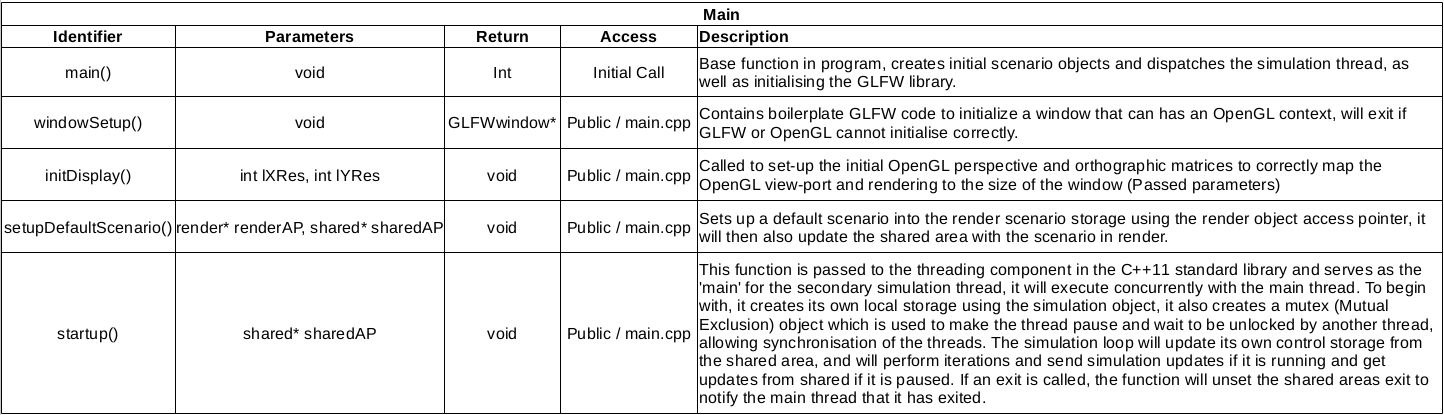
\includegraphics[width=\textwidth]{img/functions/main.png}
\end{sidewaysfigure}

\begin{sidewaysfigure}
  \subsubsection{Body}
  \centering  
  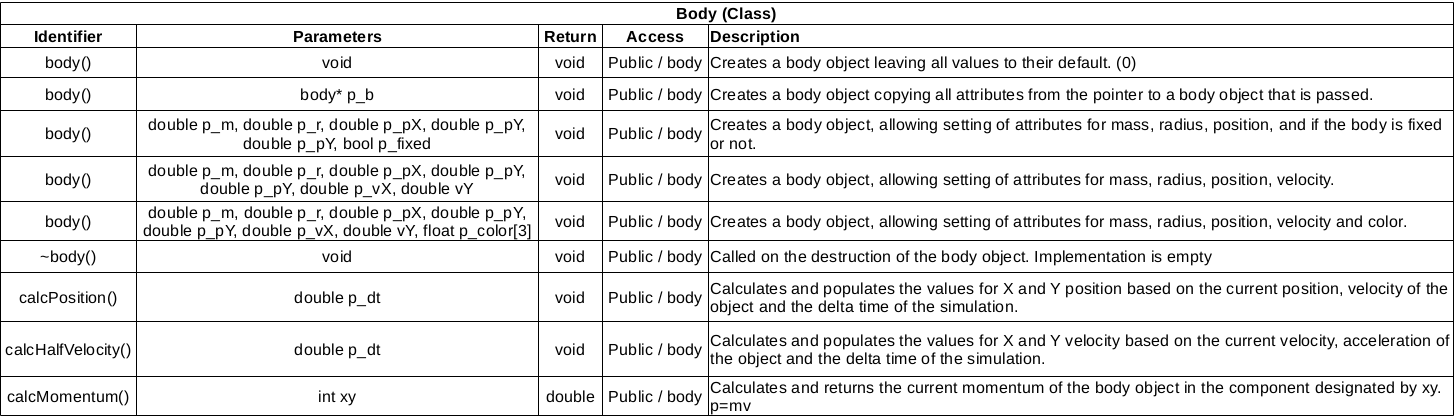
\includegraphics[width=\textwidth]{img/functions/body.png}
\end{sidewaysfigure}

\begin{sidewaysfigure}
  \subsubsection{Scenario}
  \centering  
  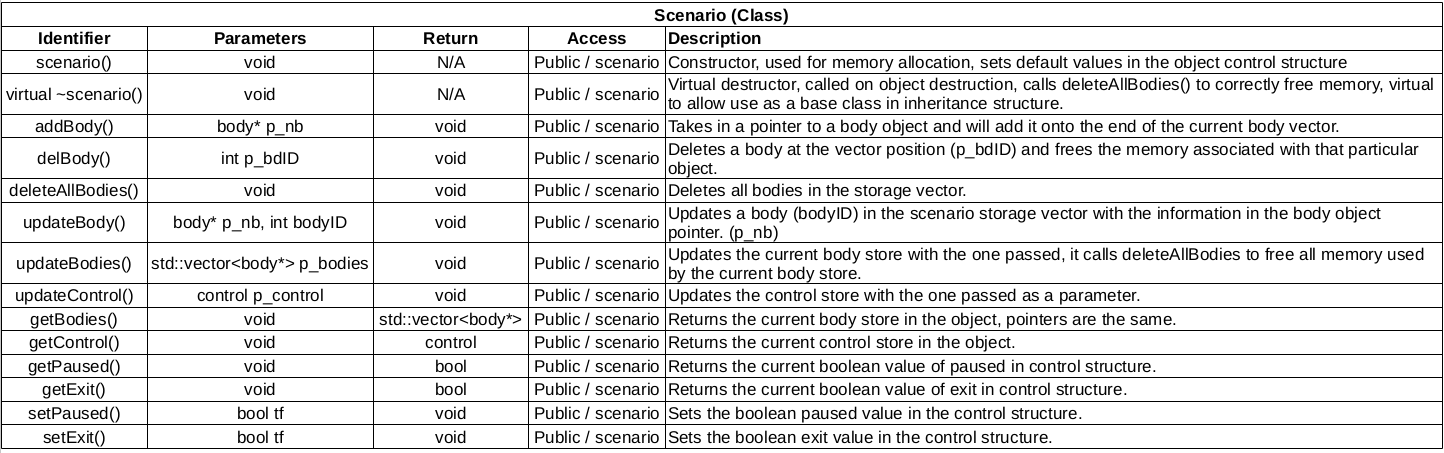
\includegraphics[width=\textwidth]{img/functions/scenario.png}
\end{sidewaysfigure}

\begin{sidewaysfigure}
  \subsubsection{Render}
  \centering  
  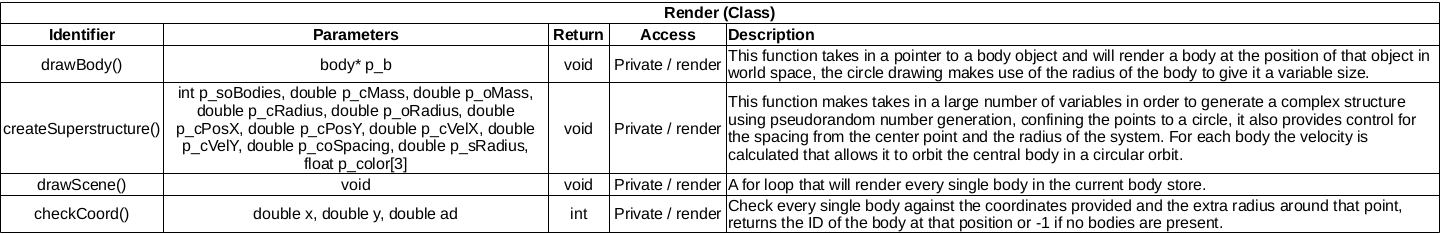
\includegraphics[width=\textwidth]{img/functions/render.png}
\end{sidewaysfigure}

\begin{sidewaysfigure}
  \subsubsection{Simulation}
  \centering  
  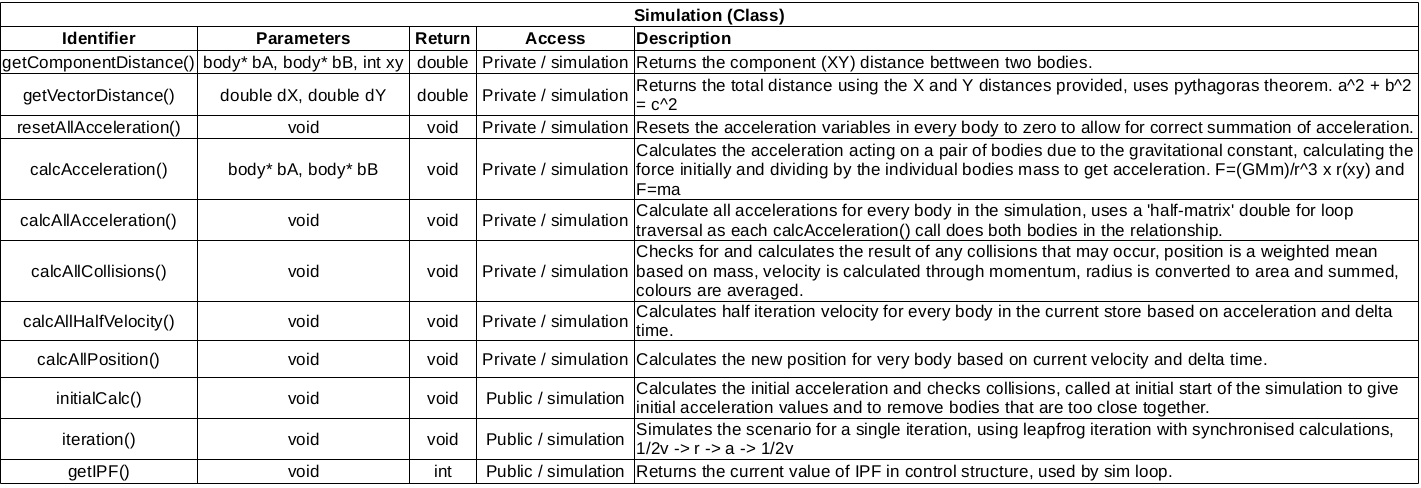
\includegraphics[width=\textwidth]{img/functions/simulation.png}
\end{sidewaysfigure}

\begin{sidewaysfigure}
  \subsubsection{Shared}
  \centering  
  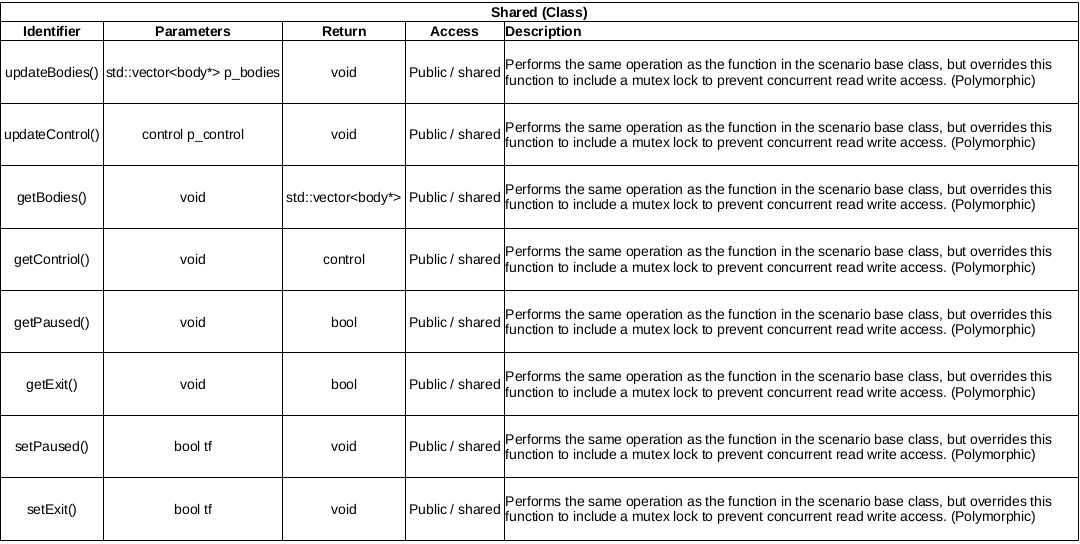
\includegraphics[width=\textwidth]{img/functions/shared.png}
\end{sidewaysfigure}

\begin{sidewaysfigure}
  \subsubsection{UI}
  \centering  
  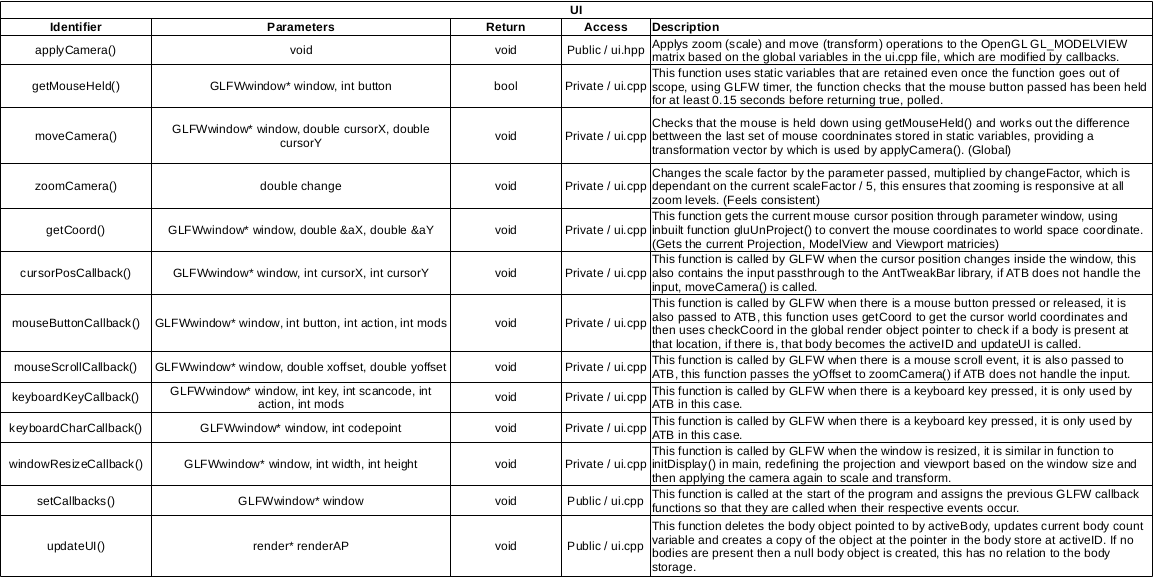
\includegraphics[width=\textwidth]{img/functions/ui.png}
\end{sidewaysfigure}

\begin{sidewaysfigure}
  \centering  
  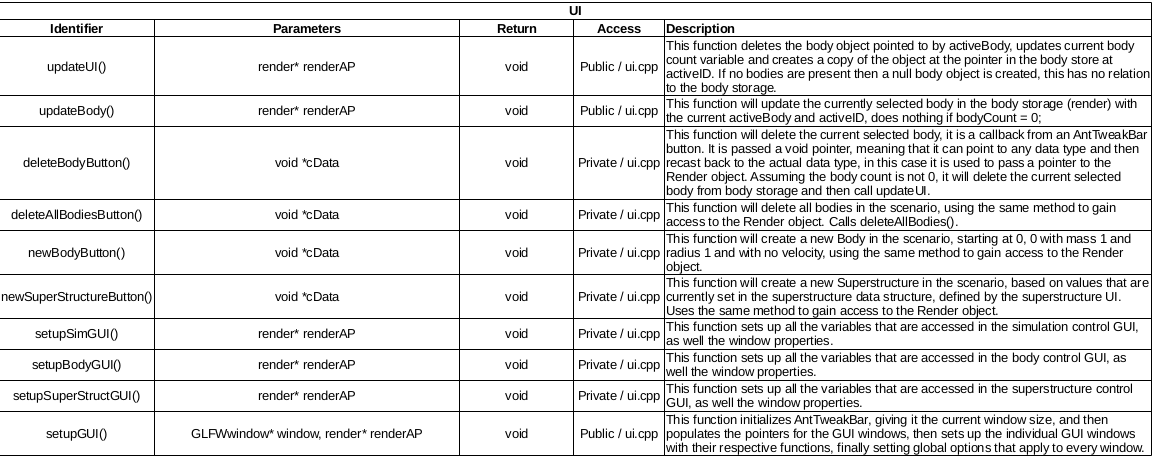
\includegraphics[width=\textwidth]{img/functions/ui2.png}
\end{sidewaysfigure}

\subsection{Variable Listing}

\begin{figure}[H]
   \centering
   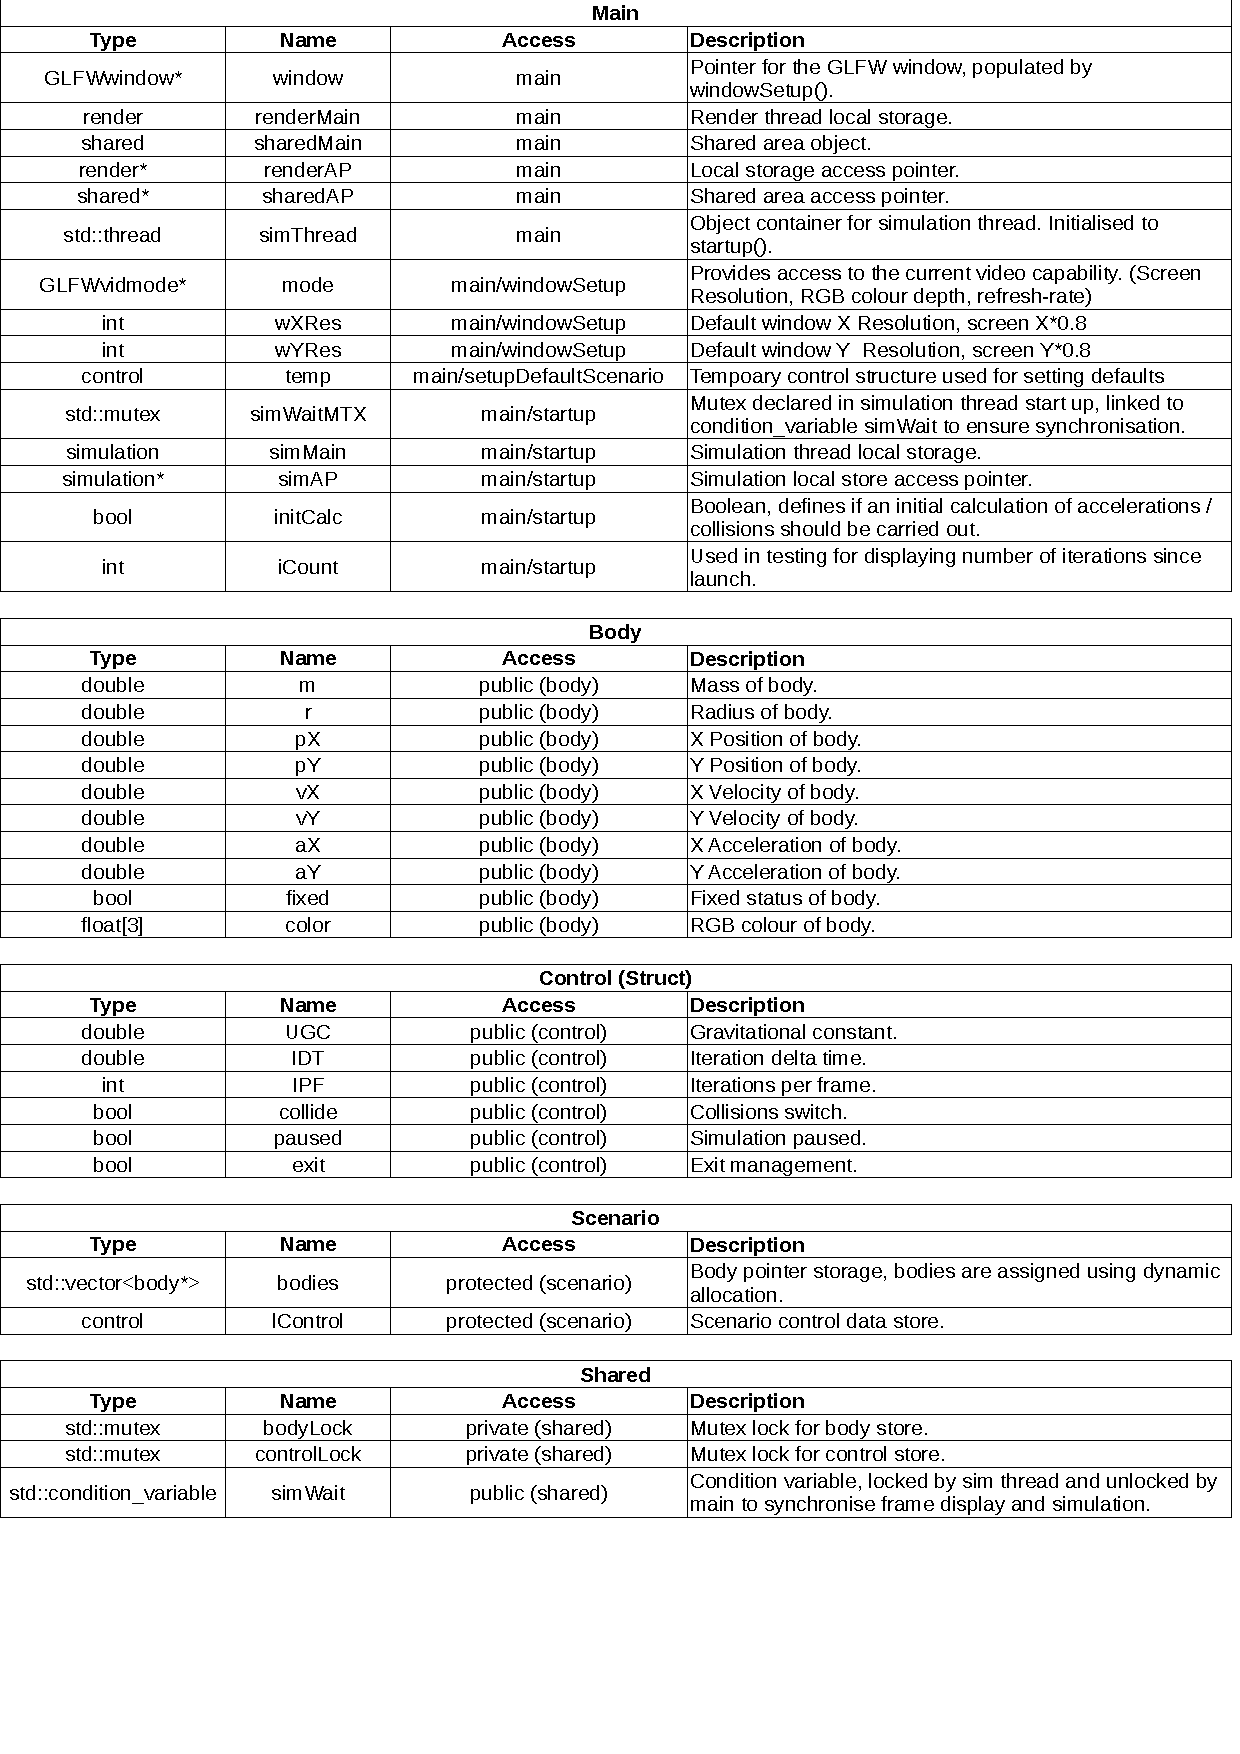
\includegraphics[page=1, width=\textwidth]{../varlist.pdf} 
\end{figure}

\begin{figure}[H]
   \centering
   \includegraphics[page=2, width=\textwidth]{../varlist.pdf} 
\end{figure}

\begin{figure}[H]
   \centering
   \includegraphics[page=3, width=\textwidth]{../varlist.pdf} 
\end{figure}